\section{準備}
本章では,本論において核となる技術内容・特徴およびそのメカニズムについて説明する.
\subsection{DNS プロトコル}
\label{sec:dns-protocol}
\subsubsection{概要}
本節では,DNS(Domain Name System)の概要について説明する.
DNSは,インターネットに接続された無数のコンピュータを一意に識別するためのIPアドレスを,人が認識しやすいドメイン名に変換するシステムである.
元来,インターネット上でのホストの識別にはIPアドレスが使用されてきた.
しかし,32bitの名前空間で10進数表記のIPv4(E.g. ``192.168.0.1")や128bitの名前空間で16進数表記のIPv6(E.g. ``2001:200:16a:8::230")は,決して人にとって認識しやすいものではない.
そこで,自然言語のようにアルファベットや数字で表記されるホスト名とIPアドレスを関連づける仕組みが登場した.
当初,hosts.txtと呼ばれる対応表は,中央集権的に管理されていた.
しかし,ホスト数の増大に伴い,管理が困難になっていく.
その解決策として登場したのが,管理するドメインをゾーンで切り出し権限を委譲していく分散的な階層構造を持つDNSである.

DNSのシステムアーキテクチャは,クライアント・サーバ構成で成り立っている.
一般に,クライアントがドメインを問い合わせた場合,サーバはドメインに対応づけているIPアドレスを応答することで,クライアントはドメインに対応づけられたIPアドレスを解決することができる.
%ドメインからIPアドレスの解決は正引きと呼ばれ,IPアドレスからドメインの解決を逆引きと呼ぶ.
DNSのサービスは,機能に応じて3つに分けられる.
\begin{itemize}
 \item Stab Resolver
 \vspace{-3mm}
 \item Full Service Resolver
 \vspace{-3mm}
 \item Authorization Server
\end{itemize}

スタブリゾルバは,名前解決の問い合わせるを依頼するクライアントノードである.
フルサービスリゾルバ(キャッシュサーバ・リカーシブサーバとも呼称される)は,スタブリゾルバからの名前解決問い合わせをハンドリングするノードである.
過去に問い合わせられた情報をキャッシュとして保持する機能と,レコード情報を保持・提供する権威サーバに対する再帰問い合わせを行う機能を担う.
一般に,フルサービスリゾルバは,``root.hints"というルート権威サーバとそのアドレスが対応づけられたファイルを保持しており,再帰問い合わせの際にはこのファイルに基づき,最初の宛先となる権威サーバのアドレスを解決する.
権威サーバは,レコード情報を保持するサーバノードであり,フルリゾルバからの転送される問い合わせ依頼に応答する.

クライアントから``www.example.com"のIPv4アドレスについて問い合わせられた場合を考える.
はじめに,クライアントであるスタブリゾルバは,スタブリゾルバと同一セグメント内のフルサービスリゾルバもしくは,ネットワークセグメントに依らずインターネット上のどのクライアントからもアクセスできるパブリックなフルサービスリゾルバ(オープンリゾルバ,パブリックリゾルバとも呼称される)に問い合わせる.
フルサービスリゾルバははじめに,ドメイン名が``www.example.com"で,リソースレコードが``A"の応答レコードがキャッシュにあるかどうかを判別する.
キャッシュにヒットした場合にはキャッシュの情報をクライアントに応答され,ヒットしなかった場合には,root.hintsファイルを参照しルート権威サーバにリクエストパケットを転送する.
クエリ(問い合わせ)を受け取ったルート権威サーバは,ルートゾーン内の``com"ドメインが委譲された権威サーバのアドレスを応答する.
次に,フルサービスリゾルバは,``com"ドメインが委譲された権威サーバに対し同様のクエリを転送する.
``com"ドメインを管理する権威サーバは,同様にして,``com"ゾーン内の``example.com"が委譲された権威サーバのアドレスを応答する.
フルリゾルバは,``example.com"ドメインを委譲された権威サーバ宛に同様のクエリを転送する.
``example.com"ゾーンを管理する権威サーバは,保持するゾーンファイルからクエリされたドメインのリソースレコードについて探索し,探索の結果としてレコード情報をフルサービスリゾルバに応答する.
フルサービスリゾルバは,権威サーバからの応答されたレコード情報のTTL(Time To Live)の期間レコード情報をキャッシュしたのち,クライアントのスタブリゾルバに結果を応答する.
このようにして,再帰的な問い合わせの仕組みに基づき名前解決がとり行われる.

\begin{figure}[h]
 \centering
 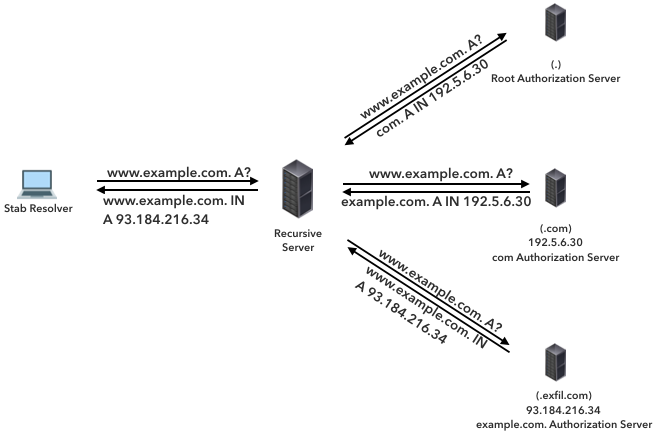
\includegraphics[width=12.0cm]{figure/dns-name-resolution.png}
 \caption{DNSによる名前解決}
 \label{fig:dns-name-resolution}
\end{figure}

\subsubsection{定義}
本節では,DNSにおける用語と概念について説明する.

ドメインは,数字とアルファベットおよびハイフン(``-")の文字列で表記され,最大長は63オクテットと定義される.
また,ドメインはルートを頂点とする階層構造で構成され,各階層にはドメインを管理する主体として権威サーバが存在し,管理主体を委譲していくことによって分散的にデータベースを管理する仕組みで動作する.

\begin{figure}[h]
 \centering
 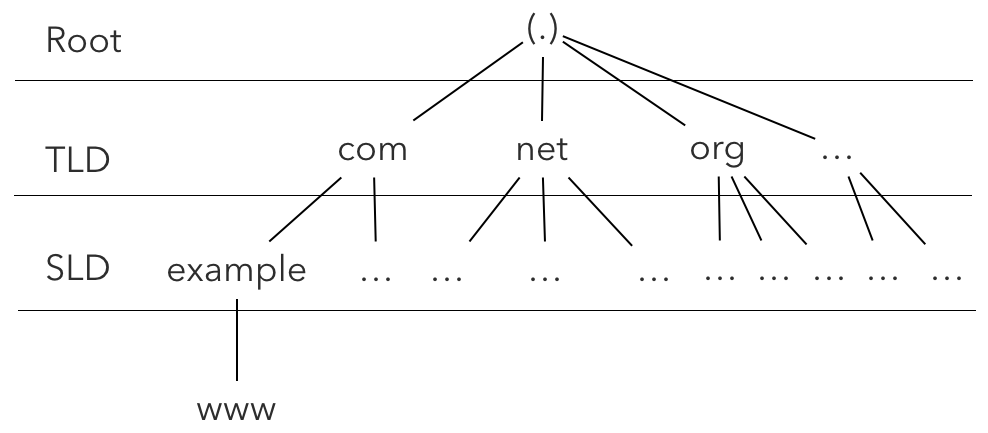
\includegraphics[width=12.0cm]{figure/dns-architecture.png}
 \caption{ドメインの名前空間}
 \label{fig:dns-architecture}
\end{figure}

ドメイン名は,ドメインに相当するラベルをドット区切りで表され,最大長は255オクテットである.
ドメイン名は右から順に階層序列が表現され,ドットで表現されるルートは一般には省略される.
最も右に位置づくラベルがTLD(Top Level Domain)であり,そのTLDからn番目(n $\mid$ n $\in$ $\mathbb{N}$)のラベルが第 n レベルドメインである.

TLDを大別すると,``.com"や``.net"をはじめとした特定分野別のgTLD(global Top Level Domain),``.jp"や``.ch"のような国ごとに割り当てられているccTLD(Co\\untry Code Top Level Domain)の二つに分けられる.

%TLDごとに登録するプロセスや必要書類,金額は異なり,上位


ドメイン名に関連づけられる情報は,リソースレコード(Resorce Record, RR)と呼ばれる.
リソースレコードは,タイプが定義されており,目的ごとに使用されるタイプが異なる.
最も一般的なレコード,Aレコードタイプは,ドメインに対してIPv4アドレスを関連づけるために使用される.
名前解決において,クライアントはドメイン名とそのドメインに関連づけられたリソースレコードを指定する.
これによって,クライアントは,ドメインに関連づけられたリソースレコード情報を取得することができる.
表~\ref{tab:resource-record}は,主要なリソースレコードである.
\begin{table}[htb]
 \centering
  \begin{tabular}{ccc}
    \toprule
		\textbf{タイプ} & \textbf{値} & \textbf{意味} \\
    \midrule
    A & 1 &  ホストのIPv4アドレス \\
    NS & 2 & 権威サーバ \\
    MF & 4 & メール転送サーバ \\
    CNAME & 5 & 別名 \\
    SOA & 6 & 権威ゾーンの開始 \\
    NULL & 10 & NULL(実験用) \\
    PTR & 12 & ドメイン名のポインター(逆引き) \\
    HINFO & 13 & ホスト情報 \\
    MINFO & 14 & メールボックスおよびメールリスト情報 \\
    MX & 15 & メール交換 \\
    TXT & 16 & 任意文字列 \\
    \bottomrule
  \end{tabular}
 \caption{主要リソースレコード一覧}
 \label{tab:resource-record}
\end{table}


%リソースレコードのタイプごとの使用頻度を知りたい


\subsection{DNS Tunneling}
本節では,DNS Tunnelingについて説明する.
DNS Tunnelingは,DNSをデータ転送のメディアとした秘匿通信手法の総称である.
第~\ref{sec:dns-protocol}節で示す通り,DNSは,ドメイン名とそのドメイン名に関連づけられたリソースレコードのレコード情報を解決するシステムであり,現代のインターネットにおいて極めて重要な役割を担うネットワークプロトコルである.
% DNSのトラフィック量
このため,DNSはトラフィックがフィルタリング・モニタリングされにくいプロトコルの一つでもある.
しかし,DNSのデザインは,クライアントサーバアーキテクチャに基づき,クライアントのスタブリゾルバと権威サーバが直接やり取りされるため,の問い合わせ情報が権威サーバに転送されるため,
転送される仕組みは,データ転送の仕組みでもある.

\subsubsection{流出メソッド : DNS Exfiltration}
\label{sec:dns-exfiltration}
DNS Exfiltrationは,DNSのクエリがDNSの再帰問い合わせの仕組みに基づいて権威サーバに到達することを利用することで,クライアントから権威サーバ方向に対してデータを転送する手法である.
一般に,組織のネットワークにセキュリティ対策を講じる時,DNSの53ポートを制限することは極端に利便性を阻害することからフィルタリング処理が施されることは少ないとされる.
DNS Exfiltrationは,上記のDNSの特性を悪用し,悪意の対象となるネットワークなどの外部との通信が制限されている環境において,外部にデータを転送する際に効果を発揮する.
過去のインシデントでは,権威サーバをデータ回収のサーバとして利用するケースや,次節~\ref{sec:dns-infiltration}の流入通信とを組み合わせて,命令サーバとの相互通信の流出方向の通信手段として利用されてきた.
この手法では,クエリを送信する主体とそのクエリを受信する権威サーバを実行者の制御下にあることを想定している.
すなわち,Exfiltrationを実施するには,予めデータの宛先となる権威サーバを動作させるために,グローバルなドメイン名を用意する必要がある.
例えば,いま,``exfil.com"というドメインを保持する権威サーバを考える.
この権威サーバは,``exfil.com"以下の全ての名前空間をゾーンとして管理することができる.
データを転送する際のキャリアとなるのは,DNSクエリの``exfil.com"以下のラベルである.
DNSのラベルは,数字・アルファベット・先頭以外でハイフン(``-")という文字列の制約があるため,任意の文字列をそのまま注入することは困難である.
そこで,ASCIIコードに変換することが可能なBase32・Base64などの文字列エンコーディングを適用させることで,文字列の制約条件を満たす.
任意の文字列を文字列エンコーディングの手法で変換させ,用意できた文字列をQNAMEに含め,適当なリソースレコードタイプを指定すれば,宛先となる権威サーバにデータが転送される.
最後に,ラベルを同一の文字列エンコーディングアルゴリズムでデコードすることで,元のデータを受け取ることができるという具合である.
このようにして,DNSの名前解決の仕組みを応用することで,任意の権威サーバに任意の文字列を転送することができる.
これがDNS Exfiltrationの動作メカニズムである.
図~\ref{fig:dns-exfiltration}に,DNS Exfiltrationのメカニズムを図解した様子である.

\begin{figure}[h]
 \centering
 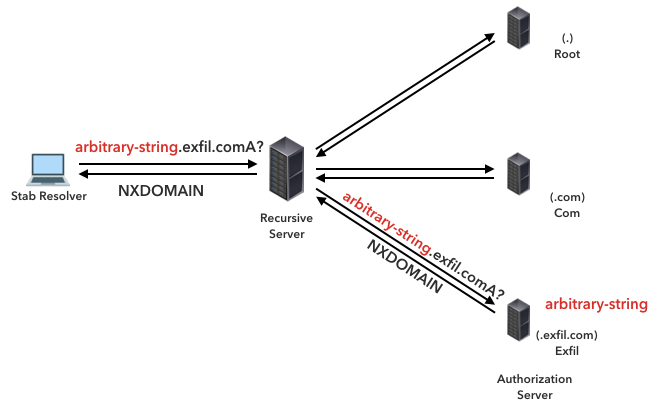
\includegraphics[width=12.0cm]{figure/dns-exfiltration.png}
 \caption{arbitrary-stringという任意の文字列が,DNSクエリのラベル部を用いて,事前に用意した権威サーバ(exfil.com)に転送される様子}
 \label{fig:dns-exfiltration}
\end{figure}

%1998年4月,DNS Tunnelingの手法は,NmapのBugtraqメーリングリストにて初めて公になったとされている\cite{bugtraq}.

\subsubsection{流入メソッド : DNS Infiltration}
\label{sec:dns-infiltration}
DNS Infiltrationは,DNS Exfiltrationと逆方向の権威サーバからクライアント方向にデータを転送する手法である.
この手法は,DNSのリソースレコードに任意の文字列が含められる設計になっていることを利用したものである.
リソースレコードのタイプは多種多様であるが,ゾーンファイルを自由に編集できる現在のDNSエコシステムでは,ドメイン名との関わりに関係なく任意の情報をドメイン名に関連づけることが可能である.
DNS Infiltrationを実施するには,送信元となる権威サーバのドメイン名に,適当なリソースレコードのタイプ(E.g. TXT)に転送したい文字列を登録しておくことで,そのドメイン名をQNAMEとしてそのレコードタイプを問い合わせることで,クライアントのもとでデータを回収することができるという具合である.
DNSのリソースレコードを転送キャリアとする流入通信のメカニズムを図解した様子が,図~\ref{fig:dns-infiltration}である.

\begin{figure}[h]
 \centering
 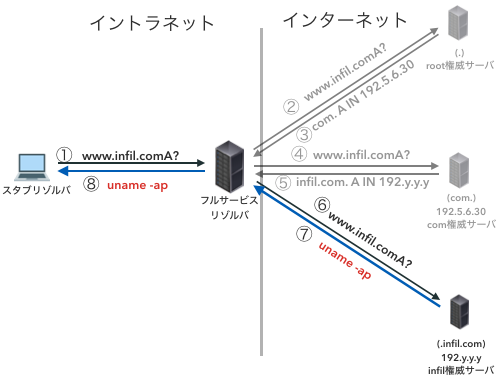
\includegraphics[width=10.0cm]{figure/dns-infiltration.png}
 \caption{TXTレコードに登録された情報について,DNSクエリで問い合わせることで権威サーバから命令情報を取得している様子}
 \label{fig:dns-infiltration}
\end{figure}


%%\subsubsection{その他課題}
%%\subsection{秘匿通信}
%%秘匿通信(英Covert Channel)とは,
%%情報転送を実現するにあたり,データの転送を本来の設計としていないプロトコルにそのデータを注入する手法である.
%%\subsubsection{ステガノグラフィ}
%%\subsubsection{代替プロトコル}
%\subsection{分散ハッシュテーブル}
%\subsubsection{アルゴリズム}
%\subsubsection{暗号学的ハッシュ関数}
%\subsection{P2P}
%\subsubsection{アーキテクチャ}
